% This file was created with tikzplotlib v0.10.1.
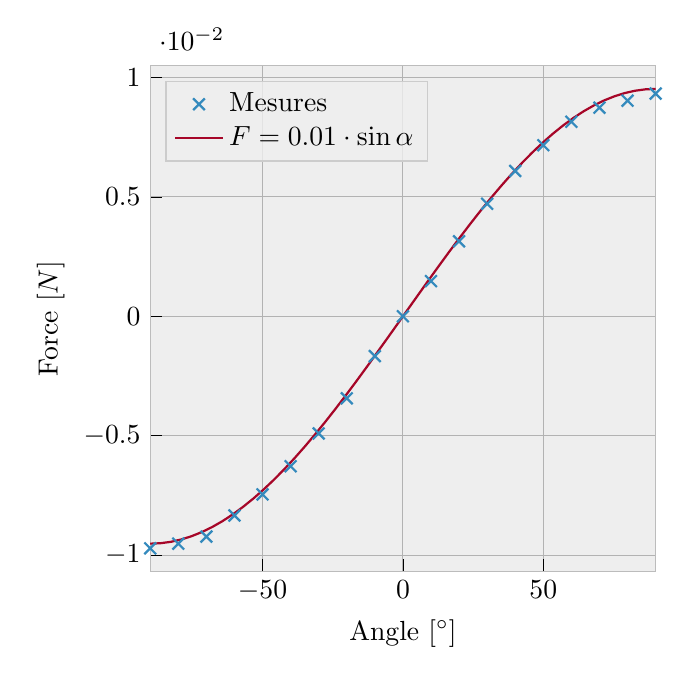
\begin{tikzpicture}

\definecolor{darkgray178}{RGB}{178,178,178}
\definecolor{firebrick166640}{RGB}{166,6,40}
\definecolor{lightgray204}{RGB}{204,204,204}
\definecolor{silver188}{RGB}{188,188,188}
\definecolor{steelblue52138189}{RGB}{52,138,189}
\definecolor{whitesmoke238}{RGB}{238,238,238}

\begin{axis}[
axis background/.style={fill=whitesmoke238},
axis line style={silver188},
height=8cm,
legend cell align={left},
legend style={
  fill opacity=0.8,
  draw opacity=1,
  text opacity=1,
  at={(0.03,0.97)},
  anchor=north west,
  draw=lightgray204,
  fill=whitesmoke238
},
tick pos=left,
width=8cm,
x grid style={darkgray178},
xlabel={Angle \(\displaystyle [^\circ]\)},
xmajorgrids,
xmin=-90, xmax=90,
xtick style={color=black},
y grid style={darkgray178},
ylabel={Force \(\displaystyle [N]\)},
ymajorgrids,
ymin=-0.0106733725254142, ymax=0.0104790230336984,
ytick style={color=black}
]
\addplot [thick, steelblue52138189, mark=x, mark size=3, mark options={solid}, only marks]
table {%
-90 -0.0097118616104126
-80 -0.00951564311981201
-70 -0.00922143459320068
-60 -0.00833845138549805
-50 -0.00745558738708496
-40 -0.006278395652771
-30 -0.00490498542785645
-20 -0.0034334659576416
-10 -0.00166773796081543
0 0
10 0.00147151947021484
20 0.00313925743103027
30 0.00470876693725586
40 0.00608217716217041
50 0.00716125965118408
60 0.00814235210418701
70 0.00873088836669922
80 0.0090252161026001
90 0.00931954383850098
};
\addlegendentry{Mesures}
\addplot [thick, firebrick166640]
table {%
-90 -0.00951755046844482
-86.326530456543 -0.0094980001449585
-82.6530609130859 -0.00943946838378906
-78.9795913696289 -0.00934207439422607
-75.3061218261719 -0.00920629501342773
-71.6326522827148 -0.0090327262878418
-67.9591827392578 -0.00882196426391602
-64.2857131958008 -0.0085749626159668
-60.6122436523438 -0.0082927942276001
-56.9387741088867 -0.00797653198242188
-53.2653045654297 -0.00762748718261719
-49.5918350219727 -0.00724709033966064
-45.9183654785156 -0.00683689117431641
-42.2448997497559 -0.00639867782592773
-38.5714302062988 -0.00593411922454834
-34.8979606628418 -0.00544512271881104
-31.2244892120361 -0.00493383407592773
-27.5510196685791 -0.0044022798538208
-23.8775501251221 -0.0038524866104126
-20.2040824890137 -0.00328707695007324
-16.5306129455566 -0.00270795822143555
-12.8571424484253 -0.00211787223815918
-5.51020431518555 -0.000913858413696289
9.18367385864258 0.00151896476745605
12.8571424484253 0.00211787223815918
16.5306129455566 0.00270795822143555
20.2040824890137 0.00328707695007324
23.8775501251221 0.0038524866104126
27.5510196685791 0.0044022798538208
31.2244892120361 0.00493383407592773
34.8979606628418 0.00544512271881104
38.5714302062988 0.00593411922454834
42.2448997497559 0.00639867782592773
45.9183654785156 0.00683689117431641
49.5918350219727 0.00724709033966064
53.2653045654297 0.00762748718261719
56.9387741088867 0.00797653198242188
60.6122436523438 0.0082927942276001
64.2857131958008 0.0085749626159668
67.9591827392578 0.00882196426391602
71.6326522827148 0.0090327262878418
75.3061218261719 0.00920629501342773
78.9795913696289 0.00934207439422607
82.6530609130859 0.00943946838378906
86.326530456543 0.0094980001449585
90 0.00951755046844482
};
\addlegendentry{$F = 0.01 \cdot \sin \alpha$}
\end{axis}

\end{tikzpicture}
